\setcounter{section}{10}

\section{Програмування синтаксичних аналізаторів}

\subsection{Синтаксична діаграма}

\textit{Синтаксична діаграма} --- це орієнтований граф, дуги котрого позначені елементами $(N \cup \Sigma)^\star$. Синтаксична діаграма будується для кожного $A$-правила КС-граматики мови програмування. \medskip

Оскільки вершини такого графа не іменуються, то вони припускаються неявно. Синтаксична діаграма позначається іменем нетермінала, для якого вона будується. \medskip

Мета побудови синтаксичних діаграм для мови програмування на основі КС-граматики:
\begin{itemize}
	\item для кожного $A$-правила КС-граматики будується синтаксична діаграма;
	\item на основі побудови синтаксичної діаграми для деякого нетермінала $A \in N$ будуємо підпрограму, яка аналізує ту частину головної програми, яку вона визначає.
\end{itemize}

Оскільки у більшості випадків при визначенні синтаксису мови програмування ми користуємося множиною рекурсивних правил, то серед підпрограм, які будуються на основі правил граматики, будуть і рекурсивні процедури (рекурсія буде як явна, так і неявна). \medskip

Сформулюємо правила побудови синтаксичного графа:
\begin{enumerate}
	\item Кожен нетермінал з відповідною множиною породжуючих правил $A \mapsto \omega_1 \mid \omega_2 \mid \ldots \mid \omega_p$, $\omega_i \in (N \cup \Sigma)^\star$, $i = \overline{1..p}$ відображається в один синтаксичний граф. \medskip

	Отже, кількість синтаксичних графів рівна кількості нетерміналів граматики $G$.

	\item Для кожного елемента слова $\omega = \alpha_1 \alpha_2 \ldots \alpha_p$, $\alpha_i \in (N \cup \Sigma)$, $i = \overline{1..p}$ будуємо ребро синтаксичного графа та покажемо його таким чином що:
	\begin{itemize}
		\item якщо $\alpha_i = x$, $x \in \Sigma$, де $x$ --- вихідна лексема, то будуємо таке ребро:
		\begin{figure}[H]
			\centering
			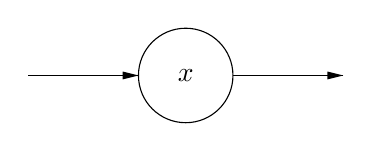
\begin{tikzpicture}[scale=0.2]
\tikzstyle{every node}+=[inner sep=0pt]
\draw [black] (0,0) circle (3);
\draw [black] (0,0) node {$x$};

\draw [black] (-10,0) -- (-3,0);
\fill [black] (-3,0) -- (-4,-.25) -- (-4,+.25);

\draw [black] (+3,0) -- (+10,0);
\fill [black] (+10,0) -- (+9,-.25) -- (+9,+.25);
\end{tikzpicture}

		\end{figure}

		\item якщо $\alpha_k = A_i \in N$ --- нетермінал граматики, то будуємо таке ребро:
		\begin{figure}[H]
			\centering
			\begin{tikzpicture}[scale=0.2]
\tikzstyle{every node}+=[inner sep=0pt]
\draw [black] (-2.5,-2.5) -- (-2.5,+2.5) -- (+2.5,+2.5) -- (+2.5,-2.5) -- cycle;
\draw [black] (0,0) node {$A_i$};

\draw [black] (-10,0) -- (-2.5,0);
\fill [black] (-2.5,0) -- (-3.5,-.25) -- (-3.5,+.25);

\draw [black] (+2.5,0) -- (+10,0);
\fill [black] (+10,0) -- (+9,-.25) -- (+9,+.25);
\end{tikzpicture}

		\end{figure}
	\end{itemize}
\end{enumerate}

Тоді, коли правило граматики $G$ має вигляд $A_i \mapsto \alpha_1 A_1 \ldots$ для побудови діаграми скористаємося обома способами:
\begin{figure}[H]
	\centering
	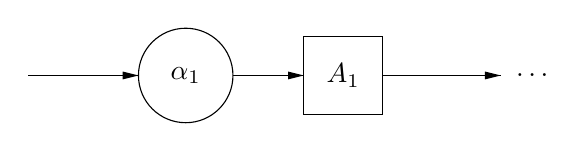
\begin{tikzpicture}[scale=0.2]
\tikzstyle{every node}+=[inner sep=0pt]
\draw [black] (-20,0) -- (-13,0);
\fill [black] (-13,0) -- (-14,-.25) -- (-14,+.25);

\draw [black] (-10,0) circle (3);
\draw [black] (-10,0) node {$\alpha_1$};

\draw [black] (-7,0) -- (-2.5,0);
\fill [black] (-2.5,0) -- (-3.5,-.25) -- (-3.5,+.25);

\draw [black] (-2.5,-2.5) -- (-2.5,+2.5) -- (+2.5,+2.5) -- (+2.5,-2.5) -- cycle;
\draw [black] (0,0) node {$A_1$};

\draw [black] (+2.5,0) -- (+10,0);
\fill [black] (+10,0) -- (+9,-.25) -- (+9,+.25);

\draw [black] (+12,0) node {$\ldots$};
\end{tikzpicture}

\end{figure}

Коли правило граматики $G$ має вигляд $A_i \mapsto \omega_1 \mid \omega_2 \mid \ldots \mid \omega_p$, то відповідний синтаксичний граф буде мати вигляд:
\begin{figure}[H]
	\centering
	\begin{tikzpicture}[scale=0.2]
\tikzstyle{every node}+=[inner sep=0pt]
\draw [black] (-20,+5) -- (-10,+5);
\fill [black] (-10,+5) -- (-11,+4.75) -- (-11,+5.25);

\fill [black] (-10,-15) -- (-9.75,-14) -- (-10.25,-14);
\draw [black] (-10,+5) -- (-10,-15);

\draw [black] (-10,0) -- (-1,0);
\fill [black] (-1,0) -- (-2,-.25) -- (-2,+.25);
\draw [black] (0,0) node {$\omega_1$};
\fill [black] (+10,0) -- (+9,-.25) -- (+9,+.25);
\draw [black] (+1,0) -- (+10,0);

\draw [black] (-10,-5) -- (-1,-5);
\fill [black] (-1,-5) -- (-2,-5.25) -- (-2,-4.75);
\draw [black] (0,-5) node {$\omega_2$};
\fill [black] (+10,-5) -- (+9,-5.25) -- (+9,-4.75);
\draw [black] (+1,-5) -- (+10,-5);

\draw [black] (0,-10) node {$\vdots$};

\draw [black] (-10,-15) -- (-1,-15);
\fill [black] (-1,-15) -- (-2,-15.25) -- (-2,-14.75);
\draw [black] (0,-15) node {$\omega_p$};
\fill [black] (+10,-15) -- (+9,-15.25) -- (+9,-14.75);
\draw [black] (+1,-15) -- (+10,-15);

\fill [black] (+10,+5) -- (+9.75,+4) -- (+10.25,+4);
\draw [black] (+10,-15) -- (+10,+5);

\draw [black] (+20,+5) -- (+10,+5);
\fill [black] (+20,+5) -- (+19,+4.75) -- (+19,+5.25);
\end{tikzpicture}

\end{figure}
де замість $\omega_1, \omega_2, \ldots, \omega_p$ будуються відповідні синтаксичні діаграми. \medskip

Якщо на основі граматики мови програмування побудована множина синтаксичних графів, то можна спробувати зменшити їх кількість, скориставшись підстановкою одних графів у інші. При цьому замість елемента $A_i$ підставляється його синтаксичний граф. Таким чином можна зменшити кількість синтаксичних графів. Для того, щоб забезпечити детермінований синтаксичний аналіз з переглядом вперед на одну лексему, потрібно накласти певні обмеження, а саме: для кожного правила $A_i$ виду  $A_i \mapsto \omega_1 \mid \omega_2 \mid \ldots \mid \omega_p$ з синтаксичною діаграмою наведеного вище вигляду необхідне виконання наступної умови: множини $\text{First}_1(\omega_j) \oplus_1 \text{Follow}_1 (A_i)$, $j = \overline{1..p}$ повинні попарно не перетинатися. Зрозуміло, що ця умова гарантує детермінований вибір шляху при русі по синтаксичній діаграмі.

\subsubsection{Код}

Подальше програмування синтаксичного аналізатора можна звести до наступних примітивів:
\begin{itemize}
	\item для фрагмента синтаксичної діаграми вигляду 
	\begin{figure}[H]
		\centering
		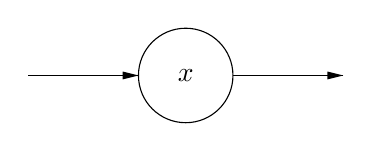
\begin{tikzpicture}[scale=0.2]
\tikzstyle{every node}+=[inner sep=0pt]
\draw [black] (0,0) circle (3);
\draw [black] (0,0) node {$x$};

\draw [black] (-10,0) -- (-3,0);
\fill [black] (-3,0) -- (-4,-.25) -- (-4,+.25);

\draw [black] (+3,0) -- (+10,0);
\fill [black] (+10,0) -- (+9,-.25) -- (+9,+.25);
\end{tikzpicture}

	\end{figure}
	відповідний фрагмент програми (наприклад, мовою С) матиме вигляд:
	\begin{verbatim}
	extern int lexem_code;  // код лексеми, яку виділив сканер
	extern char lexem_text[];  // текст лексеми
	...
	if (lexem_code == code_x) get_lexem();
	else error();
	\end{verbatim}

	\item для фрагмента синтаксичної діаграми вигляду
	\begin{figure}[H]
		\centering
		\begin{tikzpicture}[scale=0.2]
\tikzstyle{every node}+=[inner sep=0pt]
\draw [black] (-2.5,-2.5) -- (-2.5,+2.5) -- (+2.5,+2.5) -- (+2.5,-2.5) -- cycle;
\draw [black] (0,0) node {$A_i$};

\draw [black] (-10,0) -- (-2.5,0);
\fill [black] (-2.5,0) -- (-3.5,-.25) -- (-3.5,+.25);

\draw [black] (+2.5,0) -- (+10,0);
\fill [black] (+10,0) -- (+9,-.25) -- (+9,+.25);
\end{tikzpicture}

	\end{figure}
	відповідний фрагмент програми матиме вигляд:
	\begin{verbatim}
	// виклик функції, яка побудована для синтаксичної 
	// діаграми побудованої для нетермінала A_i.
	f_A_i();
	\end{verbatim}
	\item для фрагмента синтаксичної діаграми вигляду
	\begin{figure}[H]
		\centering
		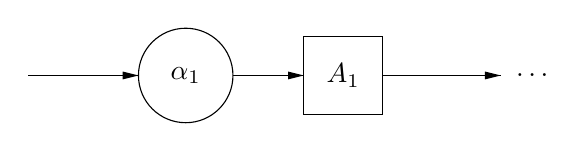
\begin{tikzpicture}[scale=0.2]
\tikzstyle{every node}+=[inner sep=0pt]
\draw [black] (-20,0) -- (-13,0);
\fill [black] (-13,0) -- (-14,-.25) -- (-14,+.25);

\draw [black] (-10,0) circle (3);
\draw [black] (-10,0) node {$\alpha_1$};

\draw [black] (-7,0) -- (-2.5,0);
\fill [black] (-2.5,0) -- (-3.5,-.25) -- (-3.5,+.25);

\draw [black] (-2.5,-2.5) -- (-2.5,+2.5) -- (+2.5,+2.5) -- (+2.5,-2.5) -- cycle;
\draw [black] (0,0) node {$A_1$};

\draw [black] (+2.5,0) -- (+10,0);
\fill [black] (+10,0) -- (+9,-.25) -- (+9,+.25);

\draw [black] (+12,0) node {$\ldots$};
\end{tikzpicture}

	\end{figure}
	відповідний фрагмент програми матиме вигляд:
	\begin{verbatim}
	extern int lexem_code;
	extern char lexem_text[];
	...
	{
	    if (lexem_code == code_alpha_1) get_lexem();
	    else error();
	    f_A_1();
	    ...
	}
	\end{verbatim}
	\item для фрагмента синтаксичної діаграми вигляду
	\begin{figure}[H]
		\centering
		\begin{tikzpicture}[scale=0.2]
\tikzstyle{every node}+=[inner sep=0pt]
\draw [black] (-20,+5) -- (-10,+5);
\fill [black] (-10,+5) -- (-11,+4.75) -- (-11,+5.25);

\fill [black] (-10,-15) -- (-9.75,-14) -- (-10.25,-14);
\draw [black] (-10,+5) -- (-10,-15);

\draw [black] (-10,0) -- (-1,0);
\fill [black] (-1,0) -- (-2,-.25) -- (-2,+.25);
\draw [black] (0,0) node {$\omega_1$};
\fill [black] (+10,0) -- (+9,-.25) -- (+9,+.25);
\draw [black] (+1,0) -- (+10,0);

\draw [black] (-10,-5) -- (-1,-5);
\fill [black] (-1,-5) -- (-2,-5.25) -- (-2,-4.75);
\draw [black] (0,-5) node {$\omega_2$};
\fill [black] (+10,-5) -- (+9,-5.25) -- (+9,-4.75);
\draw [black] (+1,-5) -- (+10,-5);

\draw [black] (0,-10) node {$\vdots$};

\draw [black] (-10,-15) -- (-1,-15);
\fill [black] (-1,-15) -- (-2,-15.25) -- (-2,-14.75);
\draw [black] (0,-15) node {$\omega_p$};
\fill [black] (+10,-15) -- (+9,-15.25) -- (+9,-14.75);
\draw [black] (+1,-15) -- (+10,-15);

\fill [black] (+10,+5) -- (+9.75,+4) -- (+10.25,+4);
\draw [black] (+10,-15) -- (+10,+5);

\draw [black] (+20,+5) -- (+10,+5);
\fill [black] (+20,+5) -- (+19,+4.75) -- (+19,+5.25);
\end{tikzpicture}

	\end{figure}
	для кожного $\omega_i$, $i = \overline{1..p}$ знайдемо множину $\text{First}_1(\omega_i) \oplus_1 \text{Follow}_1(A) = L_i = \left\{a_i^1, a_i^2, \ldots, a_i^{n_i}\right\}$. \medskip

	Оскільки за умовою $L_i \cap L_j = \varnothing$, $i \ne j$, то відповідний фрагмент програми на мові С матиме вигляд:
	\begin{verbatim}
	extern int lexem_code;
	extern char lexem_text[];
	...
	void f_A_i(void) {
	    switch(lexema_code) {
	        case code_a_1_1:
	        case code_a_1_2:
	        ...
	        case code_a_1_n_1:
	            ...  // фрагмент програми для w_1
	            break;
	        case code_a_2_1:
	        case code_a_2_2:
	        ...
	        case code_a_2_n_2:
	            ...  // фрагмент програми для w_2
	            break;
	        ...
	        ...
	        ...
	        case code_a_p_1:
	        case code_a_p_2:
	        ...
	        case code_a_p_n_p:
	            ...  // фрагмент програми для w_p
	            break;
	        default: 
	            error();
	    }
	}  // кінець функції для нетермінала A_i
	\end{verbatim}
\end{itemize}

Відмітимо, що до того, як зменшувати кількість синтаксичних діаграм шляхом суперпозиції одних діаграм в інші, необхідно знайти контексти виду $\text{First}_1(\omega_i) \oplus_1 \text{Follow}_1(A)$ для тієї синтаксичної діаграми нетермінала $A$, для якої ми виконуємо операцію суперпозиції. Ці контексти ми використаємо при програмуванні синтаксичного аналізатора на основі синтаксичної діаграми, у яку підставлено синтаксичну діаграму для нетермінала $A_i$.

\subsubsection{Одна особливість}

Досить часто при визначенні синтаксису мови програмування користуються синтаксичними правилами виду $A_i \mapsto \alpha_1 \alpha_2 \ldots \alpha_p A_i \mid \varepsilon$. Тоді синтаксична діаграма буде мати вигляд:
\begin{figure}[H]
	\centering
	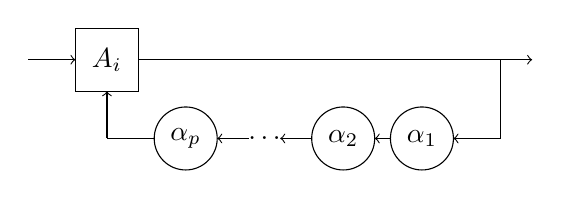
\begin{tikzpicture}[scale=0.2]
\tikzstyle{every node}+=[inner sep=0pt]
\draw [black, ->] (-5,0) -- (-2,0);
\draw [black] (-2,-2) -- (+2,-2) -- (+2,+2) -- (-2,+2) -- cycle;
\draw [black] (0,0) node {$A_i$};
\draw [black, <-] (0,-2) -- (0,-5);

\draw [black, ->] (+2,0) -- (+27,0);

\draw [black] (0,-5) -- (3,-5);

\draw [black] (5,-5) circle (2);
\draw [black] (5,-5) node {$\alpha_p$};

\draw [black, <-] (7,-5) -- (9,-5);

\draw [black] (10,-5) node {$\ldots$};

\draw [black, <-] (11,-5) -- (13,-5);

\draw [black] (15,-5) circle (2);
\draw [black] (15,-5) node {$\alpha_2$};

\draw [black, <-] (17,-5) -- (18,-5);

\draw [black] (20,-5) circle (2);
\draw [black] (20,-5) node {$\alpha_1$};

\draw [black, <-] (22,-5) -- (25,-5);

\draw [black] (+25,0) -- (+25,-5);
\end{tikzpicture}

\end{figure}

Для вище наведеної синтаксичної діаграми відповідні множини будуть: $\text{First}_1(\alpha_1 \alpha_2 \ldots \alpha_p A_i) \oplus_1 \text{Follow}_1(A_i) = L_1 = \left\{a_1^1, a_1^2, \ldots, a_1^{n_1}\right\}$. Відповідний фрагмент програми мовою С матиме вигляд:
\begin{verbatim}
extern int lexem_code;
extern char lexem_text[];
void A_i(void) {
    while (
        lexem_code == code_a_1_1 ||
        lexem_code == code_a_1_2 ||
        ... ||
        lexem_code == code_a_1_n_1
    ) {
        ...  // фрагмент програми для слова w
    }
}  // кінець підпрограми для нетермінала A_i
\end{verbatim}

Виконавши аналіз варіантів побудови синтаксичного аналізатора на основі синтаксичних діаграм, покажемо вигляд основної --- main-програми:
\begin{verbatim}
int lexem_code;
char lexem_text[1<<8];
int main () { 
    get_lexem();
    axiom();  // процедура, пов'язана з аксіомою S граматики
}
\end{verbatim}

\subsection{Контрольні запитання}

\begin{enumerate}
	\item Який граф називається синтаксичною діаграмою?
	\item Як на синтаксичній діаграмі позначаються термінали і нетермінали?
	\item Як на синтаксичній діаграмі позначаються прості (без $\vert$) і складені (з $\vert$)  правила?
	\item Напишіть фрагмент коду (наприклад на мові С) для обробки терміналів і нетерміналів.
	\item Напишіть фрагмент коду (наприклад на мові С) для обробки простих (без $\vert$) і складених (з $\vert$) правил.
	\item Як на синтаксичній діаграмі позначаються правила вигляду $A \mapsto \omega \mid \varepsilon$?
	\item Напишіть фрагмент коду (наприклад на мові С) для обробки правил вигляду $A \mapsto \omega \mid \varepsilon$.
\end{enumerate}
